\chapter{Iteration Plan}
\label{ch:iter0}

This chapter describes the iteration plan for the project, outlining how the development progresses to meet all requirements. It provides an overview of the project modules and their phased development. The execution of the project is divided into the following phases:

\begin{itemize}
    \item Midterm FYP 1
    \item Final FYP 1
    \item Midterm FYP 2
    \item Final FYP 2
\end{itemize}

\section{Midterm FYP 1}
During the Midterm of FYP 1, the primary focus was on data collection for posture detection and interview Q/A analysis. Additionally, a pre-trained model for facial expression recognition was explored and selected. The initial frontend setup and UI design were also completed in this phase, laying the foundation for further development.

\section{Final FYP 1}
By the Final FYP 1, the collected data was preprocessed for posture detection, ensuring its quality for training purposes. The pre-trained facial expression model was successfully integrated into the system. Furthermore, basic UI functionalities were developed, providing an interface for user interaction with the system.

\section{Midterm FYP 2}
The Midterm of FYP 2 focused on training the posture detection model using a hybrid approach combining MobileNetV2 and MediaPipe. The facial expression model was tested and validated to ensure its performance met the required standards. Additionally, backend development was initiated, along with API integration, enabling smooth data flow between different components.

\section{Final FYP 2}
In the Final FYP 2, the full system integration was completed, bringing together posture detection, facial expression analysis, and interview Q/A processing. Performance tuning and evaluation were carried out to enhance accuracy and efficiency. Finally, rigorous testing was conducted before deployment, ensuring that the system met all the necessary requirements.

% \begin{figure}[h] \centering 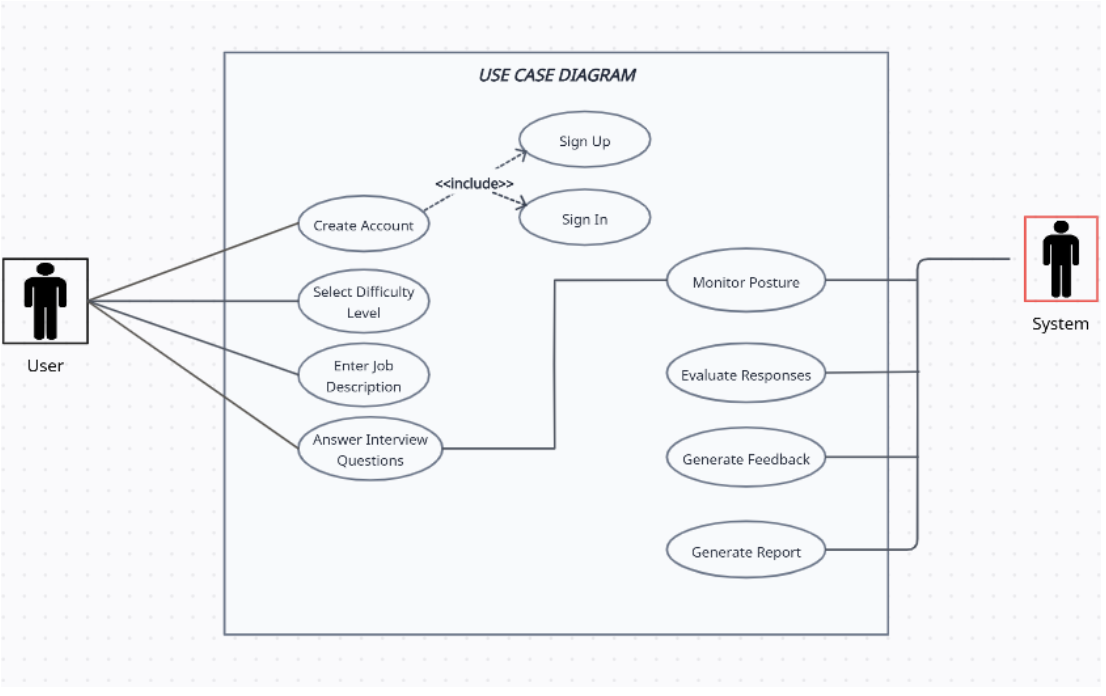
\includegraphics[width=0.5\linewidth]{sections/diagrams/UseCase.png} \caption{Use Case Diagram of the System} \label{fig
% } \end{figure}